\documentclass[12pt, a4paper]{article}
% --- MARGINS & LANGUAGE ---
\usepackage[margin=1in]{geometry}
\usepackage[english]{babel}
\usepackage[utf8]{inputenc}

% --- SPACING ---
% il corpo del testo e' a interlinea singola, non 1.5. Se il regolamento
% del corso di laurea richiede 1.5, commenta \singlespacing e scommenta
% \onehalfspacing.
\usepackage{setspace}
\singlespacing
%\onehalfspacing
%\doublespacing

% --- MATH & FONTS ---
\usepackage{amsmath}
\usepackage{amssymb}
\usepackage{mathptmx}   
\usepackage{bm}         % For bold math symbols
\usepackage{microtype}  % Improves text justification and typography

% --- FIGURES & TABLES ---
\usepackage{graphicx}
\usepackage{tabularx}
\usepackage{subfig}
\usepackage{booktabs}   % For professional looking tables
\usepackage{placeins}   % Keeps figures inside their proper sections
% NB: il pacchetto "underscore" (che permetteva di scrivere underscore  letterali nel testo senza "\_") e' stato rimosso: e' incompatibile con  le chiavi bibliografiche che contengono un underscore (es. Long_Lag2025, DeGraeve_Westermark2013) e mandava in errore silenzioso ogni \citet/\citep su quelle voci. Se ti serve un underscore letterale nel testo, scrivi "\_".

% --- CODE & UTILITIES ---
\usepackage{listings}
\usepackage{verbatim}
\usepackage{xcolor}     % serve il modello colore HTML per il rosso Padova
\usepackage[colorinlistoftodos]{todonotes}

% --- ROSSO ISTITUZIONALE UNIVERSITA' DI PADOVA ---
% Stesso colore gia' usato nelle slide (Thesis_Slides/main.tex).
\definecolor{PadovaRed}{HTML}{B20E10}

% --- CITATIONS & LINKS (VERSIONE "ROSSO PADOVA", a differenza di Lami che le ha nere) ---
\usepackage{natbib}
\usepackage[colorlinks=true, citecolor=PadovaRed, linkcolor=PadovaRed, urlcolor=PadovaRed]{hyperref}

\begin{document}

% =============================================================
% FRONTESPIZIO "IN MODALITA' PAPER" (replica dello stile dei paper:
% titolo, autore con nota a pie' pagina, data, poi abstract con
% Keywords/JEL Codes nello stesso blocco indentato)
% =============================================================
\title{The Short, the Long, and the Consequences of VAR Analysis\\ for Structural DSGE Estimation
\thanks{I am indebted to Efrem Castelnuovo for his invaluable guidance and support.}}
\author{Lorenzo Del Col\thanks{University of Padova. Contact: lorenzo.delcol@studenti.unipd.it}}
\date{October, 2026} % <- da aggiornare con la data di laurea

\maketitle
\thispagestyle{empty}

\begin{abstract}
    Truncation bias could be a severe problem regarding structural VAR analysis. 
    \citet{Long_Lag2025} claims that the role of lag choice in SVAR is crucial to correctly identify IRFs, and they claim that choosing long lags solve the bias and, 
    surprisingly, this reduce the variance of the point estimate. \citet{CEE2005} is a classic paper that studies the effects of monetary policy shock in the economy. 
    Particularly their DSGE is calibrated ex-ante using matching the model's IRFs with the ones estimated from the VAR analysis. The aim of this thesis is to perform the \citet{Long_Lag2025} exercise, 
    see if and how the IRFs changes, analys how the DSGE model calibration vary and if the model is consistent to this new empirical way to estimate the VARs. If so, we want to understand more about the 
    claimed variance reduction caused by the solution of the truncation bias how works in the Frequentist and Bayesian world.

    \vspace{0.3cm}
    \noindent\textbf{Keywords:} \todo[inline]{es. VAR, Lag Length, Truncation Bias, DSGE Estimation, Minimum Distance}

    \noindent\textbf{JEL Codes:} \todo[inline]{es. C32, C52, E32}
\end{abstract}

\newpage
\thispagestyle{empty}
\tableofcontents

\newpage
\pagenumbering{arabic}
\setcounter{page}{1}

% =============================================================
% CORPO DELLA TESI - struttura vuota su cui scrivere.
% Sottosezioni dell'Introduction ricalcano quelle di Lami
% (Main Contributions / Related Literature / Outline): tienile,
% rinominale o eliminale come preferisci.
% =============================================================

\section{Introduction}
\subsection{Research Question}

\subsection{Main Contributions}

\subsection{Related Literature}

\subsection{Outline}

\section{Theoretical Framework}

\section{Methodology}

\section{Empirical Results}

\section{Conclusion}

\clearpage

% --- BIBLIOGRAPHY ---
\bibliographystyle{apalike}
\bibliography{biblio} % Make sure you have a biblio.bib file in your project

\clearpage

% --- APPENDIX ---
\appendix
\section{Replication Files and Code}
\label{app:code}
Detail where the reader can find your code (e.g., a GitHub link).

\section{Additional Tables}
\label{app:tables}


\subsection{Implied Duration from Calvo Price Table: lags 4 8 12}

\IfFileExists{../../Output/DSGE_Parameters_Comparison/implied_duration_A4_4_8_12.tex}
    {\begin{table}[htpb]
    \centering
    \small
    \renewcommand{\arraystretch}{1.2}
    \caption{Implied Average Time between Re-Optimization}
    \label{tab:implied_duration_4_8_12}
    \begin{tabular}{lccc}
        \toprule
        \textbf{Model Specification} & \textbf{VAR $p=4$} & \textbf{VAR $p=8$} & \textbf{VAR $p=12$} \\
        \midrule

        \multicolumn{4}{l}{\textit{Homogeneous Capital Model}} \\
        Calvo parameter ($\xi_{p, hom}$) & 0.82 & 0.82 & 0.90 \\
        Implied duration (quarters)      & \textbf{5.6} & \textbf{5.6} & \textbf{9.6} \\

        \midrule
        \multicolumn{4}{l}{\textit{Firm-Specific Capital Model}} \\
        Calvo parameter ($\xi_{p, fs}$) & 0.34 & 0.64 & 0.89 \\
        Implied duration (quarters)     & \textbf{1.5} & \textbf{2.8} & \textbf{9.0} \\

        \bottomrule
    \end{tabular}

    \vspace{0.2cm}
    \raggedright
    \scriptsize{\textit{Note:} Implied duration is calculated as $D = 1/(1 - \xi_p)$.}
\end{table}
}
    {\noindent\fbox{Image Path Broken or File Missing}}

\FloatBarrier


\section{Additional Figures}
\label{app:figures}

\clearpage
\subsection{ACEL 2005 VAR Variables}
\begin{figure}[htpb]
    \centering
    \IfFileExists{../../Output/Descriptive_Statistics/Raw_Historical_Series.pdf}
    {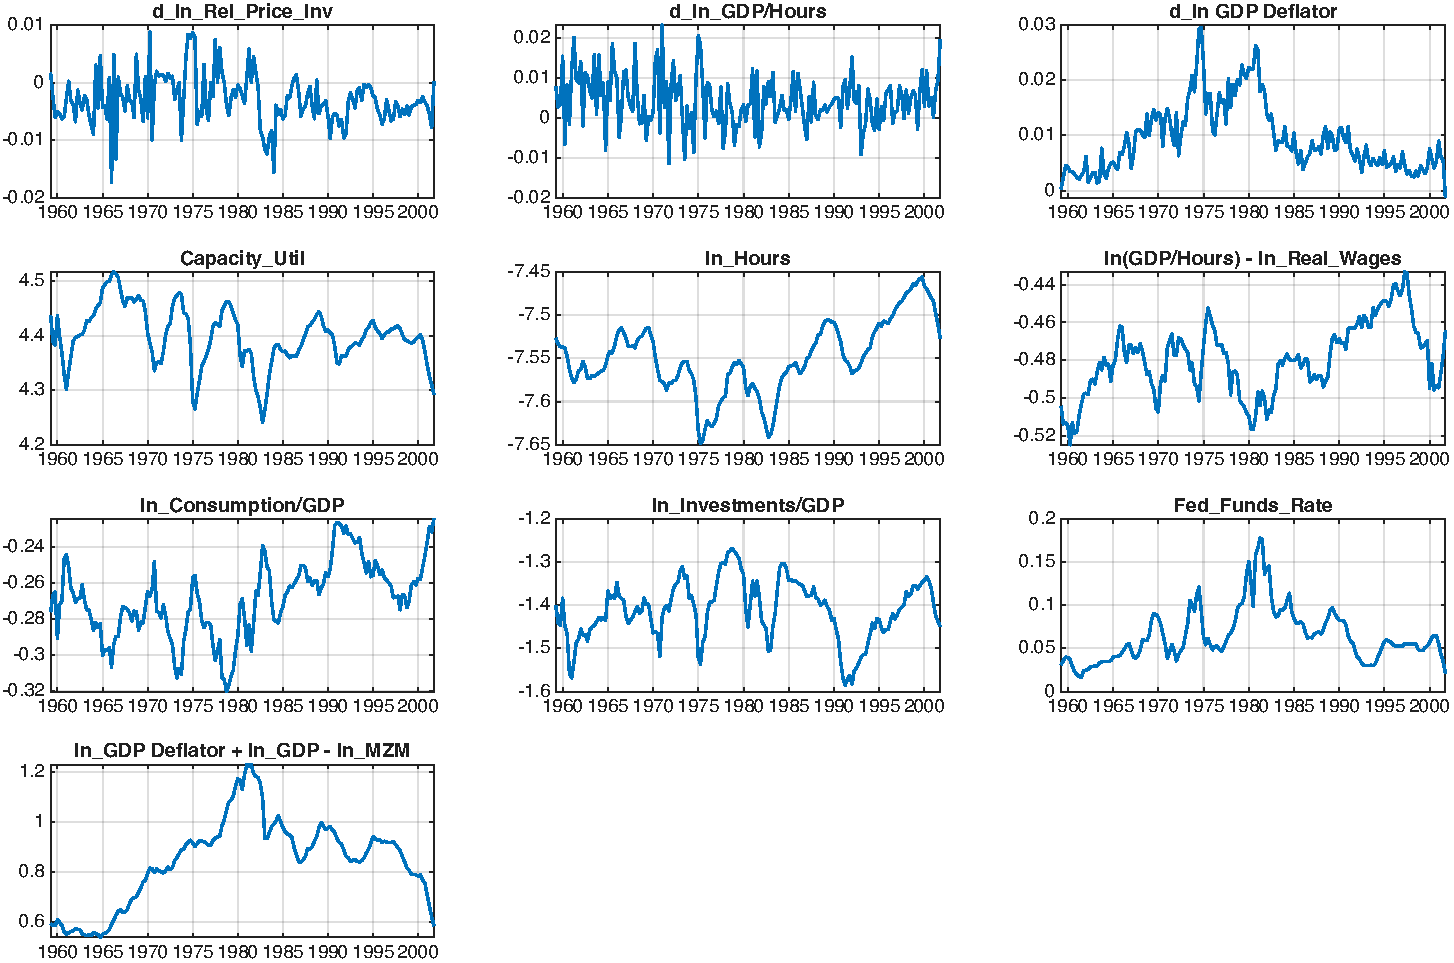
\includegraphics[width=1\linewidth]{../../Output/Descriptive_Statistics/Raw_Historical_Series.pdf}}{\fbox{Image Path Broken or File Missing}}
    \caption{Raw Historical Series}
    \label{fig:raw_series}
\end{figure}
\FloatBarrier

\end{document}
